% Überblick zur technischen Struktur des Projektes
% z.B. Aufgaben der einzelnen Roboter, Kommunikationswege (protobufs!), Übersicht zu Algorithmen und Steuerung, etc.

\chapter{Technischer Überblick}
\label{sec:ueberblick}


\section{Unterstützende Programme}
\label{subsec:ueberblick_programs}

\subsection{Git}
Zur Versionskontrolle der Software und der Diplomarbeit selber (siehe Abschnitt \ref{subsec:latex}) haben wir Git eingesetzt.
%
Das Repository ist auf GitHub, aber aktuell privat.

\subsection{Syncthing}
Zum Teilen von anderen Dateien (Weekly Reports, Zeiterfassung, etc.) zwischen Personen und Geräten
haben wir ein FOSS\footnote{Free and Open Source Software} Programm names Syncthing \cite{syncthing} genutzt.
%
Syncthing synchronisiert Dateien in einem Ordner dezentralisiert mittels Peer-to-Peer Verbindungen zwischen den Geräten.
%
Dadurch ist das Teilen von Dateien nicht von zentralisierter proprietärer Infrastruktur abhängig,
kann aber durch ``zentrale'' (und gut erreichbare) Server unterstützt werden.
%
Weiters stellt Syncthing eine rudimentäre Art der Versionskontrolle dar,
da es die Möglichkeit gibt,
bei Änderungen der Dateien eine alte Version der Datei für eine gewisse Zeit zu behalten.


Da Syncthing dezentralisiert ist,
und es somit keinen SPOT\footnote{Single Point of Truth} gibt,
kann es (selten, aber doch) zu Konflikten der Dateiversionen kommen (z.B. wenn zwei Personen die selbe Datei gleichzeitig bearbeiten). 
%
Bei solchen Konflikten erstellt Syncthing eine Kopie von einer der Versionen der Datei,
und der Nutzer muss selber entscheiden,
welche Version die ``richtige'' ist.

\subsection{Visual Studio Code}
Zur Bearbeitung der Quellcodes und der Diplomarbeit verwenden wir Visual Studio Code (auch VSC oder VSCode) mit einigen Erweiterungen.
%
Nützlich ist für uns auch die Git-Integration zur Versionskontrolle.
\begin{table}[H]
    \centering
    \begin{tabular}{r|l}
        Erweiterung         & Verwendungszweck \\ \hline
        Python              & Programmierung des Backends \\
        PlatformIO IDE      & Programmierung der Roboter \\
        vscode-proto3       & Syntax-Highlighting für Protocol Buffers \\
        LaTeX Workshop      & LaTeX Unterstützung für VSC \\
        Code Spell Checker  & Rechtschreibprüfung \\
    \end{tabular}
    \caption{Verwendete VSCode-Erweiterungen}
    \label{tab:vsc_plugins}
\end{table}
\subsection{PlatformIO}
Für die Programmierung der Mikrocontroller verwenden wir PlatformIO \cite{platformio} in Verbindung mit dem PlatformIO-Plugin für VSCode.
%
PlatformIO ist eine Alternative zur Arduino-IDE,
welche mithilfe von Plugins in viele IDEs wie z.B. VSCode oder CLion integriert werden kann.
%
Alternativ kann man PlatformIO auch über die Kommandozeile bedienen.
%
Vorteile von PlatformIO gegenüber der Arduino-IDE sind u.A. schnelleres Kompilieren,
ordentliche Auto-Vervollständigung,
statische Code-Analyse (Linting),
und ein schön geregeltes System für externe Bibliotheken.

\subsection{\LaTeX}
\label{subsec:latex}
Anstatt von WYSIWYG\footnote{What You See Is What You Get}-Editoren
wie Microsoft Word oder LibreOffice Writer verwenden wir zum Erstellen dieser Diplomarbeit
ein plattformunabhängiges Plaintext-Format namens \LaTeX.
% TODO not happy with wording above
Eine LaTeX-Datei ist (ähnlich wie Markdown) einfach nur eine Textdatei mit zusätzlichen Befehlen.
Deshalb können wir \texttt{.tex}-Dateien sehr gut mit Versionskontrollsoftware wie Git verwenden
und somit genau Änderungen rückverfolgen und gegebenenfalls zurücksetzen.
%
Weiters können wir mit LaTeX unsere Arbeit in mehrere Dateien aufteilen,
was das Ganze um einiges übersichtlicher macht.
%
Der größte Vorteil von LaTeX ist aber wohl,
dass die Formatierung einheitlich für den Nutzer übernommen wird,
sodass sich dieser besser auf den Inhalt konzentrieren kann.
%
Wenn man aber dann doch mal selber etwas anders formatieren will,
ist das mit LaTeX durch die Verwendung von Textbefehlen
aber immer noch schneller als in MS Word zur Maus zu greifen
und sich durch GUIs durchzuklicken.

\section{Funktionsbeschreibung}
\label{subsec:funktionsbeschreibung}

\subsection{Guide}
Der Guide hat die Aufgabe,
mit dem nachgerüsteten LiDAR-Sensor die Umgebung nach Hindernissen abzusuchen.
%
Hierbei ist allerdings zu beachten,
dass der Guide die Datenverarbeitung nicht selbständig durchführt,
sondern die rohen Sensordaten einfach an das Backend weiterleitet.
%
In diesem Kontext sind Tamerlan und Bambi also nichts anderes als Hindernisse.

\subsection{Tamerlan \& Bambi}
Tamerlan und Bambi sind ``blind'' im dem Sinne,
dass sie über keine Sensoren zur Hinderniserkennung verfügen.
%
Sie sind komplett von Anweisungen des Backends abhängig.

\subsection{Backend}
Das Backend ist das ``Gehirn'' des Projekts.
%
Es empfangt die LiDAR-Daten vom Guide,
verarbeitet sie,
und sendet Befehle an die Roboter.
%
Die LiDAR-Daten und die Ergebnisse der Verarbeitung werden auch
über eine Websocket-Verbindung ans Frontend weitergeleitet.
%
Außerdem empfängt es die Sensordaten der Gyroskope und Accelerometer der Roboter, und auch ans Frontend weiter. 
%
Gegebenenfalls empfängt das Backend auch Befehle vom Frontend, und leitet diese an die Roboter weiter.

\subsection{Frontend}
Das Frontend empfängt Sensordaten vom Backend und stellt diese dar.
%
LiDAR-Daten werden auf einer Karte dargestellt,
auf der auch die Ergebnisse der Hinderniserkennung am Backend zu sehen ist.
%
Die Daten der Gyroskope und Accelerometer werden in einem sich laufend aktualisierendem X/Y Diagramm dargestellt.
%
Zusätzlich gibt es im Frontend die Möglichkeit für Nutzer,
einen oder mehrere Roboter auf manuelle Steuerung umzuschalten,
und diese(n) dann fernzusteuern.
%
Das Frontend ist eigentlich zum autonomen Betrieb nicht nötig,
es wird nur für Debugging-Zwecke und menschliche Intervention benötigt.

\subsection{Kommunikationswege}
\label{subsec:ueberblick_comms}
\& Beschreibung
\begin{figure}[H]
    \centering
        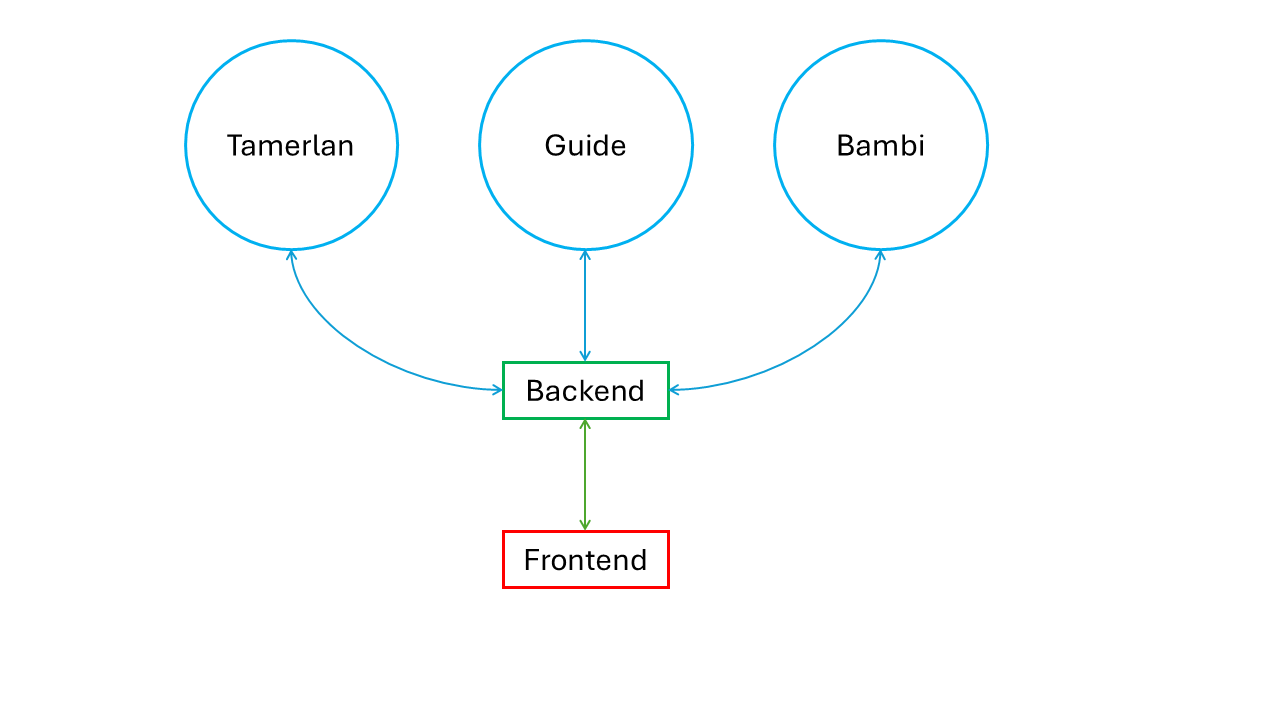
\includegraphics[width=\textwidth, center]{img/Kommunikationswege.png}  
    \caption{Kommunikationswege}
    \label{fig:kommunikationswege}
\end{figure}

\section{Protocol Buffers}
\label{subsec:ueberblick_protobufs}
Protocol Buffers \cite{protobufs} (``protobufs'') sind ein binäres Übertragungsformat,
welches von von Google entwickelt und veröffentlicht wurde.
%
Gegenüber Datenformaten wie JSON und XML gibt es drei wesentliche Vorteile:
\begin{enumerate}
    \item Da Protocol Buffers auf Binärdaten anstatt von Text basieren,
    ist die Übertragung viel effizienter \cite{7765670}.
    %
    Insbesondere bei der Verwendung mit Mikrocontrollern ist das ein enormer Vorteil.

    \item Bei Protocol Buffers gibt es explizit definierte Datenstrukturen.
    %
    Diese Datenstrukturen sind (bei korrekter Verwendung) mit älteren Versionen rückwärts-kompatibel.

    \item Für wie Verwendung mit unterschiedlichen Programmiersprachen kann (und soll) man aus protobuf-Definitionen
    Wrapper-Bibliotheken generieren.
    %
    Diese Wrapper-Bibliotheken können ohne weiteren Aufwand direkt verwendet werden,
    um auf die Datenstrukturen zuzugreifen.
\end{enumerate}

\subsubsection{Effizienz}
Wie schon oben erwähnt erreichen Protocol Buffers,
insbesondere bei kleinen Nachrichten,
einen viel kleineren Overhead als textbasierte Formate wie JSON oder XML.
%
% Quelle: https://protobuf.dev/programming-guides/encoding/
TODO mehr infos; Tatsächlicher Vergleich mit Zahlen.


\subsubsection{Datenstrukturen}
TODO

\subsubsection{Wrapper-Bibliotheken}
TODO

\section{Sensoren}
\label{subsec:ueberblick_sensors}

\subsection{LiDAR}
\label{subsec:ueberblick_lidar}

\subsection{Gyroskop}
Jeder der drei Roboter ist mit einem Gyroskop/Accelerometer vom Typ \texttt{MPU6050} ausgestattet.
%
Dieser Sensor ist bereits im originalen Tumbller-Kit inkludiert, also ist die Installation entsprechend einfach.
%
Der \texttt{MPU6050} versorgt den Mikrocontroller über I2C mit Messdaten zu drei Gyroskop- und drei Accelerometerachsen.
%
Diese Informationen werden dann vom Mikrocontroller verwendet, um den Roboter aufrecht zu halten.
%
Weiters leitet der Mikrocontroller die Daten zur weiteren Verarbeitung bzw. Analyse für Debugging-Zwecke an den zentralen Server weiter.

\subsection{Drehgeber}
\label{subsec:ueberblick_rot_enc}
In den im Tumbller-Kit mitgelieferten Motoren ist bereits ein Drehgeber mit eingebaut,
welcher mit Hall-Sensoren funktioniert.
%
Mit diesem Drehgeber kann die aktuelle Motorgeschwindigkeit als Feedback zur Motorsteuerung gemessen werden.
%
Die Impulse des Drehgebers werden auf eine gewisse Zeitspanne im Format zusammengefasst und dann regelmäßig an den Server weitergeleitet.